There is a family of four conceptual models for RBAC security policy, which define the various dimensions of it~\cite{PTN2009}. $RBAC_0$ is considered as the basic model, which has the minimum requirements for a system.  Whereas, $RBAC_1$, $RBAC_2$ and $RBAC_3$ are more advanced models.  However, the latter models are based on the basic one, $RBAC_0$, as some elements are common for all types of models~\cite{AhHu2007}.

$RBAC_0$ contains some basic elements of RBAC policies, where cannot define any RBAC policy without specifying those elements.  Usually, components of $RBAC_0$ are Users (U), Roles (R), Permissions (P), Sessions (S) as well as relationships between them. In addition to the components of $RBAC_0$, $RBAC_1$ model supports the concept of Role Hierarchy (RH).  Hierarchical of roles describe the gradualism of authorizations and responsibilities in an organization.  In other words, RH is about defining what are called senior roles (more powerful roles) and junior roles (less powerful roles), where senior roles may inherit permissions that are assigned to junior roles.

\begin{figure}[bht]
\centering
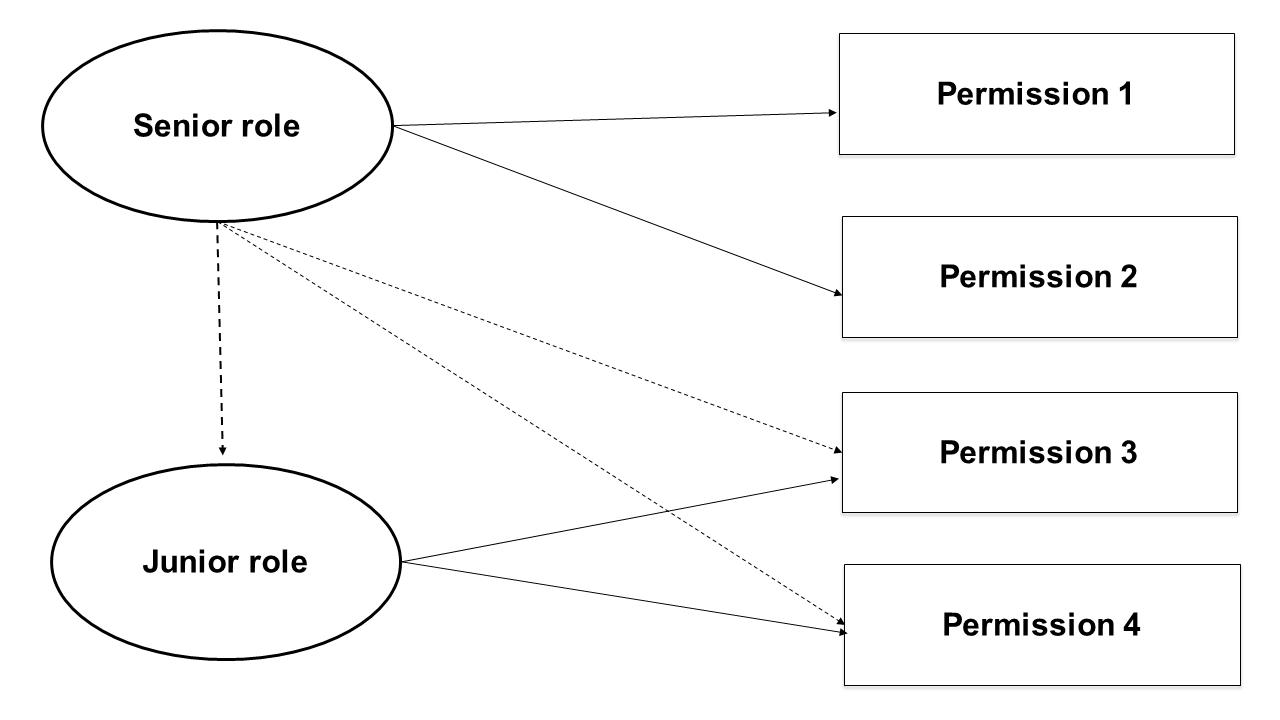
\includegraphics[scale=0.26]{RolesHierachy.png}
\caption{Role Hierarchy.}
\label{fig:RBACPol}
\end{figure}

In order to provide a powerful protection to the RBAC-based systems, $RBAC_3$ (constraints model) is defined to be the main drive of RBAC security policies.  That is $RBAC_3$ uses a mechanism to force restrictions and form a high level security policy.  Constraints can be applied to any relationship/assignment that has been defined in the two previous models, such as UA, PA, Sessions and Role Hierarchy (RH) (see Figure~\ref{}).  There are many types of applicable constraints, in particular those which deal with exclusiveness of roles (Separation of Duties) and cardinality constraints.


\begin{figure}[bht]
\centering
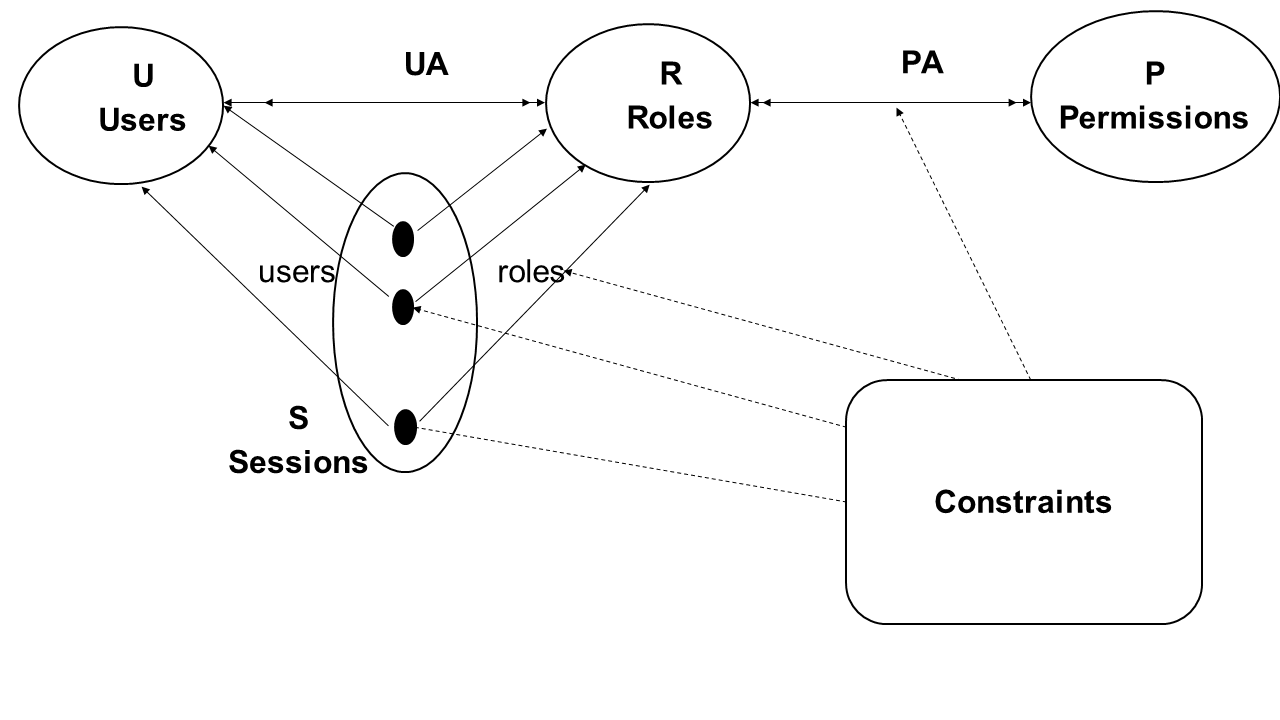
\includegraphics[scale=0.26]{modelConstraints.png}
\caption{RBAC Model Constraints.}
\label{fig:RBACPol}
\end{figure}

Mutual exclusiveness of roles is one of the most common constraints for an RBAC model.  Usually, it is defined as Separation of Duties (SoD), where the same user cannot be assigned to two conflicted roles at the same time~\cite{FeKu2009}.  For example, for two roles R1 and R2 belonging to mutually exclusive sets of roles, then if a user U is assigned to R1, this implies that U cannot be assigned to R2, and vice versa.  This is expressed formally as:
  
 
\begin{align*} 
If&  (U \times R1) \in UA \Rightarrow  (U \times R2) \notin UA ;     and \\
If&  (U \times R2) \in UA \Rightarrow (U \times R1) \notin UA
\end{align*}    


Cardinality constraints define the maximum number of users that can be assigned to a particular role.  Likewise, cardinality constraints can be used to specify the number of roles that can be related to a particular user.  In addition to that, they can be applied to Permission Assignment (PA) for the purpose of restricting the number of permissions that a particular role should be assigned to~\cite{SDAG2008}.


